\chapter{Sprint 3}
\label{chap:S4}

In the third sprint of the project the user feedback had been collected from the workshop held in Oslo. The main focus of the sprint was on Pre-delivery efforts both by working on the system development while most of the resources were focused on writing the report. Based upon the user feedback the group made some changes to the design and functionality of the prototype. The group's main goal was getting all the documentation ready for the pre-delivery, while part of the development team worked on the planned Android app. The group had also reached the point where adding more features might be too time consuming. The goal is delivering a functioning web page rather than one with many half-working functions.

\section{Sprint plan}
\label{sec:S4Plan}

Since feedback had been collected from end users at the workshop in Oslo, the group started working on suggestions given by users. The most important decision was whether to start the creation of a mobile app, as this had been the feature that had been most in demand by the end users. Regardless of whether a mobile app would be created, the back-end for picture uploads had to be completed. Meetings would keep focusing on discussing user feedback, and which parts we could and could include in the scope of this project, and what would be considered further work to be done by others at a later time. In the end we decided the added usability of having a mobile app meant we needed one and we decided to make an application with functionality limited to uploading pictures. This, along with other decisions made based on the feedback, will be discussed further in section \ref{sec:S4DesignImpl} and \ref{subsec:S4RetrospectiveGroupDynamics}.

\paragraph{} Much of the group had to focus on getting everything ready for the pre-delivery, and this would become more important as the sprint went on. As we phased more people over from implementation to working on the report and pre-delivery, we left the two most experienced developers doing work on the intended mobile application.

\paragraph{} We would also have a session in the right use of YouTrack, which included everyone taking the time to insert time they had spent on tasks in the backlog, in order to get a burndown chart of the work we had already done.

\begin{figure}[ht!]
  \centering
  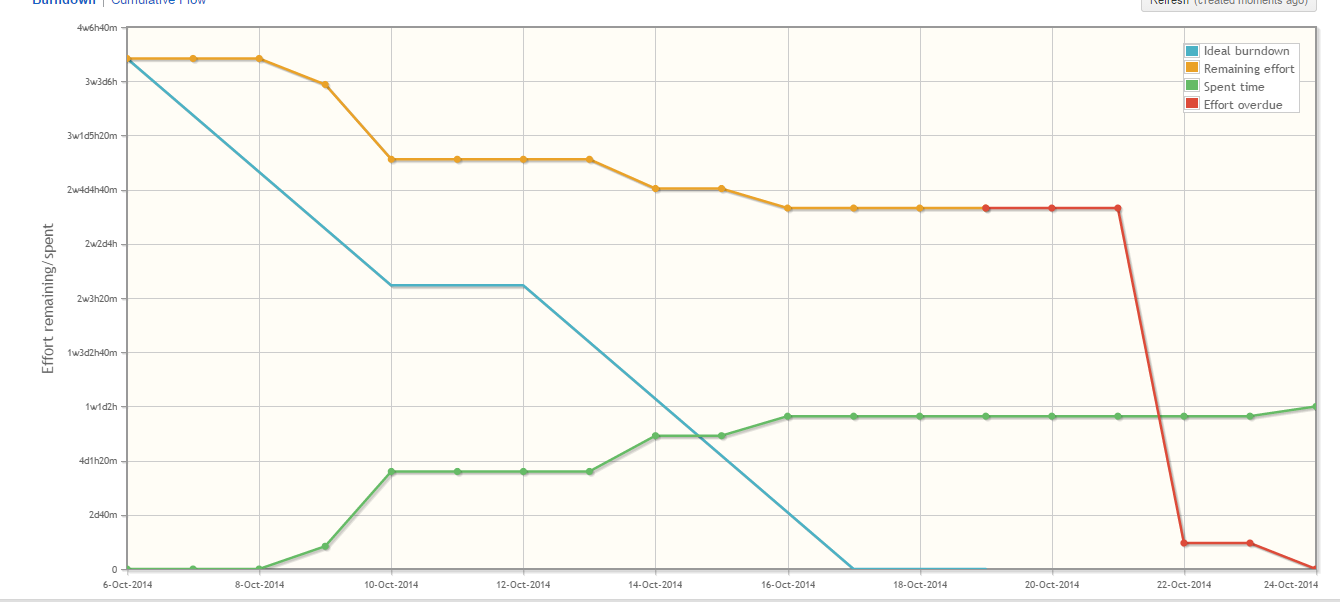
\includegraphics[width=\linewidth]{./Sprint4/img/burndown}
  \caption{Burndown chart for Sprint 3.}
  \label{fig:S4PlanBurndown}
\end{figure}

\section{Duration and workload}
\label{sec:S4Duration}

\begin{minipage}{\linewidth}
\centering
\setlength{\tabcolsep}{22pt}
\textbf{Sprint 3:} 
\smallskip
\rowcolors{1}{blue!20}{blue!10}
\begin{tabular}{ |l l| }
	\hline
	\it{Duration} & 2 weeks \\
	\it{Start} & October 6th \\
	\it{End} & October 19th. \\
	\it{Workload} & Hours spent by the entire group on Sprint 3. \\
	\it{Goal} & 40 - 50 hours per person \\
	\hline
\end{tabular}
\end{minipage}\\%
%
\begin{minipage}{\linewidth}
\setlength{\tabcolsep}{15pt}
\centering
\rowcolors{1}{blue!20}{blue!10}
\begin{tabular}{ |l|l| }
	\hline
	\multicolumn{2}{|c|}{\cellcolor{gray!25} Workload} \\
	\hline
	\it{Planning} & 77 hrs\\
	\it{Development} & 83 hrs\\
	\it{Design} & 16 hrs\\
	\it{Documentation} & 106 hrs\\
	\it{Testing} & 6 hrs\\
	\it{Learning} & 2 hrs\\
	\hline
	\textbf{\textit{Total Workload}} & 290 hrs\\
	\hline
\end{tabular}
\captionof{table}{Workload of Sprint 3.} 
\end{minipage}

The group managed its target at 20.7 hours per person per week this sprint, and things were going very well. There were still things we could do better, and we aimed to keep improving our work.

\section{Sprint backlog}
\label{sec:S4Backlog}
\begin{minipage}{\linewidth}
\setlength{\tabcolsep}{12pt}
\centering
\rowcolors{1}{blue!20}{blue!10}
\begin{tabular}{|p{1cm}|p{4cm}|p{2cm}|p{2cm}|}
\hline
\multicolumn{4}{|c|}{\cellcolor{gray!25} Backlog for Sprint 3 part 1} \\
\hline
\cellcolor{gray!25} ID & \cellcolor{gray!25} Description & \cellcolor{gray!25} Estimated Time & \cellcolor{gray!25} Actual Time \\
\hline
CDP-26 & Create basic Android app to browse Alternative Spaces. Initial focus on upload of pictures with possibility to extend to browse entire site by embedding a browser in the app. & 2w & 1w1d2h30m \\
CDP-23 & Create the database table for the event. This is a design task, so think of all the fields that we need to describe an event, f.ex. time, location, title, description, interests, etc. & 2h & 2h \\ 
RPT-3  & Report pre-delivery, to be delivered to the supervisor. By no means are these the completed finished versions, and they will not be graded  & 1d6h & 2d9h30m \\
\hline
\end{tabular}
\captionof{table}{Backlog for Sprint 3.} 
\end{minipage}\\%
%
\begin{minipage}{\linewidth}
\setlength{\tabcolsep}{12pt}
\centering
\rowcolors{1}{blue!20}{blue!10}
\begin{tabular}{|p{1cm}|p{4cm}|p{2cm}|p{2cm}|}
\hline
\multicolumn{4}{|c|}{\cellcolor{gray!25} Backlog for Sprint 3 part 2} \\
\hline
\cellcolor{gray!25} ID & \cellcolor{gray!25} Description & \cellcolor{gray!25} Estimated Time & \cellcolor{gray!25} Actual Time \\
\hline
CDP-27 & \it{A "page" within the AS Android app that has a button to upload. Should be possible to: Take picture and upload it without going via gallery} & 4d & 4d2h \\
CDP-28 & \it{Add a basic form that forwards the sign in credentials to back end. If credentials are valid, perhaps store them locally?} & 1d & 4h30m \\
CDP-38 & \it{Make it possible to upload picture from the gallery.} & 4h & 4h \\
CDP-40 & \it{Add checks to deal with when location and/or Internet service is unavailable (F.ex. display error message)} & 4h & 2h \\
RPT-4 & \it{Write the abstract, consult the technical writing presentation if in doubt, 0.5 page~ish} & 1h & 45m \\
RPT-5 & \it{Write introduction} & 2h & 5h \\
RPT-6 & \it{Our pre-study. Should be obvious} & 6h & 7h \\
RPT-7 & \it{Justification of choice of lifecycle model} & 4h & 7h \\
\hline
\end{tabular}
\end{minipage}

\section{Design and implementation}
\label{sec:S4DesignImpl}

As mentioned in section \ref{sec:S4Plan}, the early parts of this sprint focused a lot on how the feedback from end users would change our design.

\paragraph{} The most important feedback from the workshop was the necessity of a mobile application. Since many young people in the T\o yen area do not have a personal computer, only a phone, it would be difficult to get youth interested in the web page if they did not have a good way to upload pictures to the site themselves.
\subparagraph{} The group had originally decided on only a web page as the platform of choice for this project, with a mobile app considered something that could be discussed as an important future development. With this new feedback, especially the fact computers might not be an option for many kids in the area the prototype would be tested in, however, we needed a serious discussion of the possibility for a mobile app. The group realized that the picture uploading had to be developed anyway, and as far as the back end was concerned, mobile or web did not matter much. Brage had experience developing apps for Android, and he was of the opinion that developing a limited app, for example focusing on picture uploads only, was definitely possible within our time-frame.
\subparagraph{} In the end, since getting people to upload pictures was such a core feature in the project, a mobile app seemed like the only good choice. We decided that development this sprint would focus on designing a limited app for uploading photos to the page. The results are seen in figure \ref{fig:S4DesignImplAppStart} and \ref{fig:S4DesignImplAppUpload}.

\begin{figure}
\begin{minipage}{.45\linewidth}
	\centering
    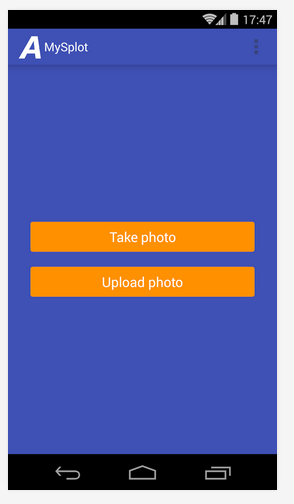
\includegraphics[width=.8\linewidth]{./Sprint4/img/appStart.png}
    \caption{Start screen for the application}
    \label{fig:S4DesignImplAppStart}
\end{minipage}%
\hspace{0.1\linewidth}
\begin{minipage}{.45\linewidth}
	\centering
    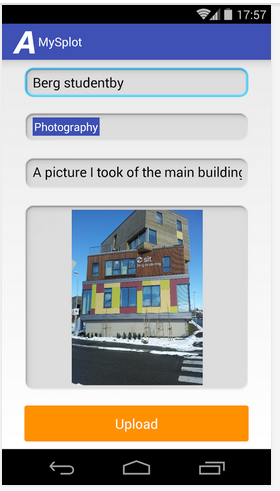
\includegraphics[width=.8\linewidth]{./Sprint4/img/appUpload.png}
    \caption{Upload screen for the application}
    \label{fig:S4DesignImplAppUpload}
\end{minipage}

\end{figure}

\paragraph{} There was also some work done on the back-end for events. This was done in preparation for implementing event creation and viewing in the next sprint.

\paragraph{} The group managed to mostly finish the Android application, which was a very good result considering that most people had to focus on the pre-delivery. All items in the backlog were finished. All that was left was some bug fixing, and the group was ready for event creation and other work on the website next sprint.

\section{Testing and results}
\label{sec:S4Testing}

Since no branches were merged into the master branch this sprint, no integration testing was needed. The testing focused on the Android application. Testing was usually done straight after a change to the app, by testing every required operation after the new code had been added, and bug fixing proceeded immediately after finding a bug, with focus shifting from feature introduction to fixing the problem at hand. On the back-end, testing was done on the tables to make sure they were correct.

\begin{figure}
    \centering
    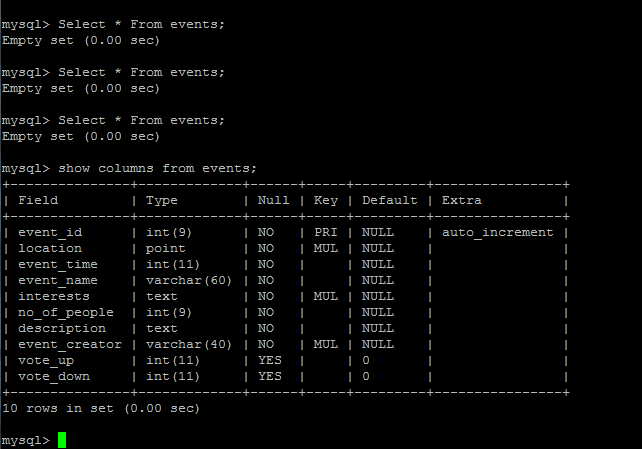
\includegraphics[width=100mm]{./Sprint4/img/eventTable}
    \caption{Event database table.}
    \label{fig:S4TestingEvent}
\end{figure}

\begin{figure}
    \centering
    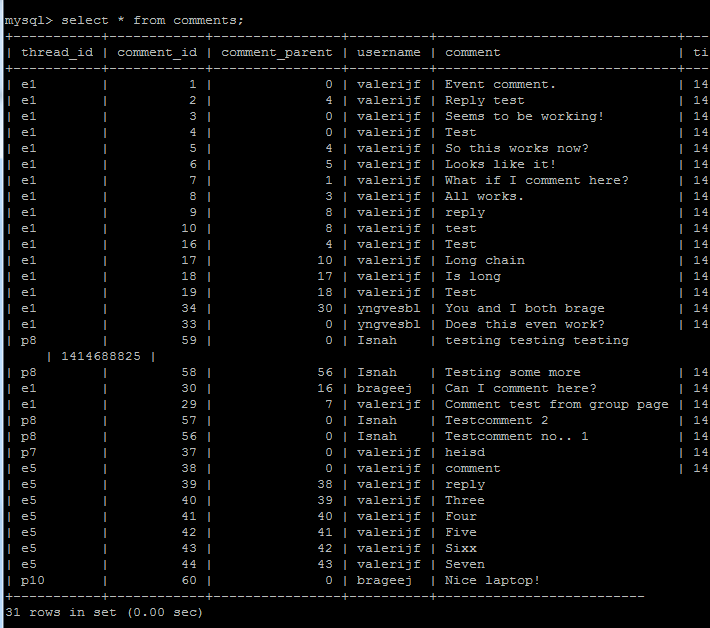
\includegraphics[width=\linewidth]{./Sprint4/img/commentsDB}
    \caption{Testing comments in the database.}
    \label{fig:S4TestingComments}
\end{figure}

\section{Sprint retrospective}
\label{sec:S4Retrospective}

%TODO !!!!!!!!!!!!!!!!!!!!!!!!!!!!!!!!!!!!!!!!!!!!!!!!!!!!!!!!!!!!!!!!!!!!!!!!!!!!!!!!!!!!
%TODO !!!!!!!!!!TOTAL REWRITE ALERT !!!!!!!!!!!!!!!!!!!!!!!!!!!!!!!!!!!!!!!!!!!!!!!!!!!!!!
%TODO !!!!!!!!!!!!!!!!!!!!!!!!!!!!!!!!!!!!!!!!!!!!!!!!!!!!!!!!!!!!!!!!!!!!!!!!!!!!!!!!!!!!

\subsection{Start doing}
\label{subsec:S4RetrospectiveStart}

\begin{itemize}
   \item Move more people from development to the report.
   \item Keep YouTrack up to date.
   \item Learn LaTeX to write directly to the report.
   \item Get the report into LaTeX instead of Google Docs.
\end{itemize}

\subsection{Stop doing}
\label{subsec:S4RetrospectiveStop}

\subsection{Continue doing}
\label{subsec:S4RetrospectiveContinue}

\begin{itemize}
    \item Continue system development.
    \item Keep the work summary up to date and well written.
    \item Work together to be able to ask questions.
    \item Make changes based on user feedback.
    \item Add bugs to YouTrack.
    \item Fix any bugs you are able to.
\end{itemize}

\subsection{Group Dynamics}
\label{subsec:S4RetrospectiveGroupDynamics}

The amount of work done went up even further this sprint, and we finally reached the group's goal of over 20 hours per week for each member. We managed to implement the Scrum methodology better, with retrospectives at the meetings, and a good overview of what was being done using YouTrack.

\paragraph{} The biggest challenge this sprint was the change in design for the project. With the new scope including an Android application. Because of the feedback, we had to find a way to fit this new plan into our time-frame, and we decided to make the app very high priority, and rather push less important features out of the scope of the project, rather than deliver a prototype with a core feature that would not be easily used by the target audience.

\paragraph{} As mentioned in chapter \ref{chap:S2}, there were many other changes also suggested at the presentation in Oslo. We spent a lot of time discussing which of these changes we would implement and which were either put off to future work, or scrapped entirely. Suggestions that were put off will be discussed further in chapter \ref{chap:Further} along with our own thoughts regarding important features we did not have time to add.

\paragraph{} Other than the lack of a mobile application, the second most important feedback was regarding the size of the map in the photos screen on the web page. The end users found it too small, which made it difficult to navigate, and the lack of an ability to search for locations by address was also a drawback. We decided that both of these were important changes to make. Neither would take too much time, and it was an important layer of polish for the prototype. Sharing to other social media was also considered a simple thing to add to the page to make those functionalities we had more polished. Much of the early part of the next sprint was spent discussing different ways of responding to some of the other feedback from users.

\subsection{Customer Feedback}
\label{subsec:S4RetrospectiveFeedback}

The customer seemed very impressed to see the mobile application at the end of the sprint, since we had made it fairly clear earlier in the project that a such an app would not be within the scope of our project. Since we made it clear that the project would not be more than a prototype when we finished, they asked us to write a comprehensive list of ideas for further work that could be done, to help them move forward and get a complete system.



%TODO ORIGINAL STUFF NOT PLACED YET! As the User feedback has been collected from the workshop held in Oslo, the group started working on the suggestions given by users, modifications for the previous system with  some changes in Search Map display, Events should be displayed in the map as well as in the feed when selected, Pictures (and other media) should display some information when selected, like interests, location and maybe the uploader, When registering as a new user you should be automatically logged in, Should have a mobile app that integrates the phone's camera to enable one-click upload, Enable support for some kind of direct user to user messaging, Consider some way of connecting this to Facebook (sharing photos), Needs some form of reward for use, like meeting new friends and getting feedback when people interact with your content (Like button/user rating),They suggested us the following tips for creating exposure for the product by
% Ads on T-banen,
% Help from affiliated teenagers,
% Cooperation with existing sites focused on youth, Ung Info,
% Advertise the qualities that make this product unique,
% keep in mind how to stimulate and create user habits to check this thing often.
% The users suggested that the current solution for uploading pictures-
% Taking a picture in mobile, connecting the mobile to Personal Computer(PC),transferring and % uploading the picture into web is very inefficient and off-putting,
% Needs system to remove troublesome users: administrators/moderators,
% Some way to invite some other users or notify them of an activity in order to not be completely alone if no one comes.
%The group considered most of the suggestions and part of the development team started working with the Android app for enabling users to upload a picture into website from the mobile.
%The group has decided to make changes with the previous designed web pages for the Map and within the Event Creation page to add a location search map.
%There was a session upon the use of YouTrack, whole team has been explained upon how to assign the Tasks, estimated hours and fill the hours of work accomplished for particular task and decided to update YouTrack by filling up all the previous work of everyone from the team, so the threshold of work will be shown upon the “Burn down chart”.


%TODO MOVE TO SPRINT 5?
%Changes in search map - two input fields for address and interests
%Design: design of map window has to be recreated/reviewed
%Task: Everyone should be viewed by username
%Event Creation form
%Feature: Connecting with Facebook-used for sharing
%Feature: Location should have a map